%% This is file `elsarticle-template-2-harv.tex',
%%
%% Copyright 2009 Elsevier Ltd
%%
%% This file is part of the 'Elsarticle Bundle'.
%% ---------------------------------------------
%%
%% It may be distributed under the conditions of the LaTeX Project Public
%% License, either version 1.2 of this license or (at your option) any
%% later version.  The latest version of this license is in
%%    http://www.latex-project.org/lppl.txt
%% and version 1.2 or later is part of all distributions of LaTeX
%% version 1999/12/01 or later.
%%
%% The list of all files belonging to the 'Elsarticle Bundle' is
%% given in the file `manifest.txt'.
%%
%% Template article for Elsevier's document class `elsarticle'
%% with harvard style bibliographic references
%%
%% $Id: elsarticle-template-2-harv.tex 155 2009-10-08 05:35:05Z rishi $
%% $URL: http://lenova.river-valley.com/svn/elsbst/trunk/elsarticle-template-2-harv.tex $
%%
\documentclass[preprint,authoryear,12pt]{elsarticle}

%% Use the option review to obtain double line spacing
%% \documentclass[authoryear,preprint,review,12pt]{elsarticle}

%% Use the options 1p,twocolumn; 3p; 3p,twocolumn; 5p; or 5p,twocolumn
%% for a journal layout:
%% \documentclass[final,authoryear,1p,times]{elsarticle}
%% \documentclass[final,authoryear,1p,times,twocolumn]{elsarticle}
%% \documentclass[final,authoryear,3p,times]{elsarticle}
%% \documentclass[final,authoryear,3p,times,twocolumn]{elsarticle}
%% \documentclass[final,authoryear,5p,times]{elsarticle}
%% \documentclass[final,authoryear,5p,times,twocolumn]{elsarticle}

%% if you use PostScript figures in your article
%% use the graphics package for simple commands
%% \usepackage{graphics}
%% or use the graphicx package for more complicated commands
%% \usepackage{graphicx}
%% or use the epsfig package if you prefer to use the old commands
%% \usepackage{epsfig}

%% The amssymb package provides various useful mathematical symbols
%%\usepackage{amssymb}
\usepackage{amsmath}
\usepackage{amssymb}
%%\setmathfont[range={\mathcal}]{Lucida Calligraphy}

%% The amsthm package provides extended theorem environments
%%\usepackage{amsthm}

%% The lineno packages adds line numbers. Start line numbering with
%% \begin{linenumbers}, end it with \end{linenumbers}. Or switch it on
%% for the whole article with \linenumbers after \end{frontmatter}.
%% \usepackage{lineno}

%% natbib.sty is loaded by default. However, natbib options can be
%% provided with \biboptions{...} command. Following options are
%% valid:

%%   round  -  round parentheses are used (default)
%%   square -  square brackets are used   [option]
%%   curly  -  curly braces are used      {option}
%%   angle  -  angle brackets are used    <option>
%%   semicolon  -  multiple citations separated by semi-colon (default)
%%   colon  - same as semicolon, an earlier confusion
%%   comma  -  separated by comma
%%   authoryear - selects author-year citations (default)
%%   numbers-  selects numerical citations
%%   super  -  numerical citations as superscripts
%%   sort   -  sorts multiple citations according to order in ref. list
%%   sort&compress   -  like sort, but also compresses numerical citations
%%   compress - compresses without sorting
%%   longnamesfirst  -  makes first citation full author list
%%
%% \biboptions{longnamesfirst,comma}

% \biboptions{}

\journal{Control Engineering Practice}

\begin{document}

\begin{frontmatter}

%% Title, authors and addresses

%% use the tnoteref command within \title for footnotes;
%% use the tnotetext command for the associated footnote;
%% use the fnref command within \author or \address for footnotes;
%% use the fntext command for the associated footnote;
%% use the corref command within \author for corresponding author footnotes;
%% use the cortext command for the associated footnote;
%% use the ead command for the email address,
%% and the form \ead[url] for the home page:
%%
%% \title{Title\tnoteref{label1}}
%% \tnotetext[label1]{}
%% \author{Name\corref{cor1}\fnref{label2}}
%% \ead{email address}
%% \ead[url]{home page}
%% \fntext[label2]{}
%% \cortext[cor1]{}
%% \address{Address\fnref{label3}}
%% \fntext[label3]{}

\title{Dynamic Modelling, Simulation, and Model Predictive Control of a Tailings Treatment Surge Tank}

%% use optional labels to link authors explicitly to addresses:
%% \author[label1,label2]{<author name>}
%% \address[label1]{<address>}
%% \address[label2]{<address>}

\author{J. J. Burchell$^{a, b}$}
\author[pretoria]{D. le Roux}
\author[pretoria]{I. K. Craig}

\address[sibanye]{Sibanye-Stillwater, Johannesburg, South Africa}
\address[pretoria]{Department of Electrical, Electronic and Computer Engineering, University of Pretoria, Pretoria, South Africa.}

\begin{abstract}
%% Text of abstract
A dynamic model is derived to describe the rate of change of both volume and density for a tailings treatment surge tank. This model is validated using data from one of Sibanye-Stillwater's plants that stabilises tailings fed to a chrome recovery plant. Using the model simulations are was used to develop a non-linear model predictive controller for the plantsimulate the surge tank's response to multiple input density disturbances while under linear model predictive control. Compared to a simple control philosophy that relies only on a sizeable surge tank inventory to dampen input density disturbances, the model predictive controller was able to reduce output density fluctuations by a further $17$ $\%$.
\end{abstract}

\begin{keyword}
%% keywords here, in the form: keyword \sep keyword
dynamic modelling \sep simulation \sep model predictive control

%% MSC codes here, in the form: \MSC code \sep code
%% or \MSC[2008] code \sep code (2000 is the default)

\end{keyword}

\end{frontmatter}

%\linenumbers

%% main text
%===============================================================================
%///////////////////////////////////////////////////////////////////////////////
\section{Introduction}\label{sec:background}
Waste material from the primary processing of a metal ore is called tailings, and are typically stored in a dam formed by constructing a barrage from the tailings itself. The barrage is constructed at an angle for structural support, resulting in the dam taking on a trapezoidal shape. 

In hard rock mining tailings consists of a fine particle slurry. When deposited in the dam the solids from the slurry settles to the bottom, and the water is recycled back to the process. To accomodate more waste the height of the dam is increased by extending the crest of the barrage.  

In general, tailings are retreated to recover metals or minerals with sufficient economic value, to reclaim valuable land, or to mitigate safety and environmental risks. This paper discusses the implementation of a non-linear model predictive controller (NMPC) to increase the recovery of chrome from a platinum group metals (PGM) tailings. This PGM tailings is owned and retreated by Sibanye-Stillwater in the Marikana area in the North West province of South Africa.

The development of the NMPC followed the general control problem (GCP) framework for developing advanced controllers \citep{Craig1997, CraigAndHenning2000}, outlined in Fig. \ref{fig:GeneralControlFramework}. The layout of this paper also follows the GCP framework. In section \ref{sec:CircuitAnalysis} the tailings retreatment circuit is studied for control purposes. A mathematical model is developed and validated in section \ref{Section:DynamicModelling}. Using this model, a control design and analysis is performed in section \ref{sec:ControllerDesignAndSimulation}. An NMPC was implemented, and its performance is evaluated in section \ref{sec:ControllerImplementationAndEvaluation}.

\begin{figure}[h!]
	\centering
	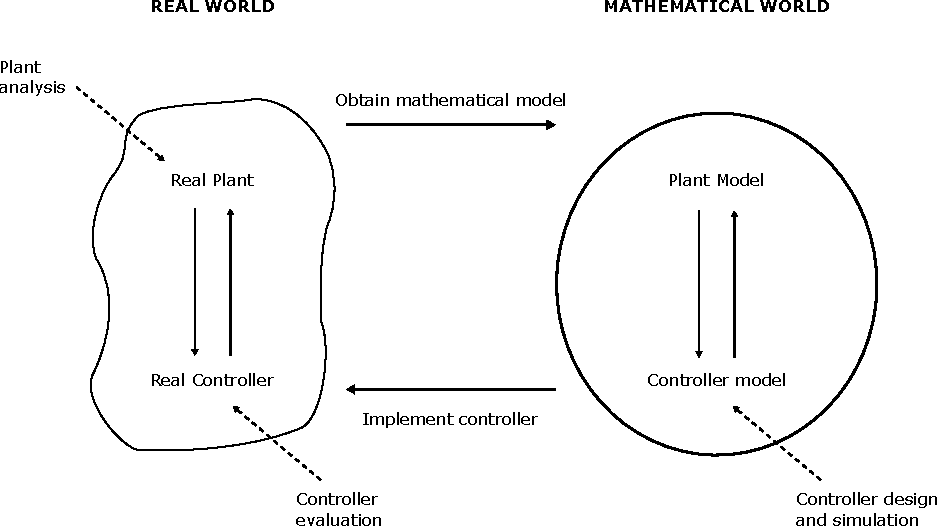
\includegraphics[width=5.2in]{GeneralControlFramework.pdf}
	\caption{The general control framework for developing advanced control systems.}
	\label{fig:GeneralControlFramework}
\end{figure}

\section{Circuit Analysis}\label{sec:CircuitAnalysis}
%///////////////////////////////////////////////////////////////////////////////
Fig. \ref{fig:ChromeRecoveryFlowsheet} presents an overview of the circuit used to recover chrome from the tailings dam. A bulk tailings treatment (BTT) plant dewaters and stabilises the tailings before it is fed to a chrome concentrator plant. This concentrator plant produces chrome using spiral separators, which sort the tailings into different chrome grades and a gangue waste product using gravity separation. 
 
To assess the feasibility of this tailings retreatment project, and to motivate for its funding, the following factors were likely considered:
\begin{itemize}
	\item The total amount of chrome in the dam, estimated from a geolocial survey.
	\item Characteristics of the tailings, such as its particle size distribution (PSD), also estimated by a geolocical survey.
	\item What recovery\footnote{Here \emph{recovery} refers to the percentage of chrome in the tailings that would be recovered as product, with all unrecovered chrome lost to the gangue waste.} would be achieved by the project. The recovery of the project would be influenced by tailings characteristics, such as the PSD, which would affect the efficiency of cyclones and spirals. 
	\item What would be the operating throughput\footnote{Here \emph{throughput} refers to the rate, in tons per hour, at which tailings would be processed by the circuit.}, which would largely be influenced by design considerations such as the sizing of pumps, spirals, thickeners, etc.
	\item The expected chrome price over the life of the project.
	\item The operating costs over the life of the project.
\end{itemize} 

Using these factors an internal rate of return (IRR), an estimate of the profitability of the project, can be estimated.  If the internal rate of return (IRR) for the project exceeds some minimum acceptable rate of return the project is deemed feasible.

Of the listed factors influencing the IRR, recovery is by far the most affected by improving the control and operation of the circuit post its commissioning. The total amount of chrome in the dam, the tailings characteristics, and chrome price can not be influenced at all, while operating cost and throughput is largely influenced by circuit design. The key performance indicator for the chrome retreatment circuit is therefore its recovery. During the lifetime of the project, operations are continuously under pressure to achieve a target recovery, and any improvements on this recovery is celebrated as a realisation of the upside potential for the project.

Ultimately, the recovery of the circuit depends on the efficiencies of the spiral separators, since they are the classifiers, sorting tailings into chrome product and gangue waste. Since the spiral separators' efficiencies are most sensitive to disturbances in density \citep{HollandBatt1982}, the key control objective for the circuit must be to supply the chrome concentrator with a stable feed density.

\begin{figure}[h!]
	\centering
	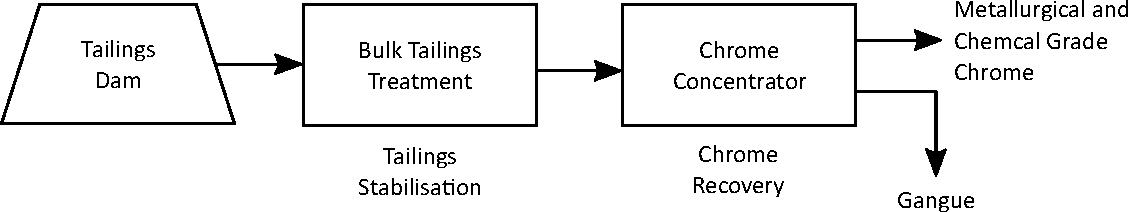
\includegraphics[width=5.2in]{ChromeRecoveryFlowsheet.pdf}
	\caption{Chrome recovery circuit.}
	\label{fig:ChromeRecoveryFlowsheet}
\end{figure}
%###
Fig. \ref{fig:TailingsDam} presents an overview of the tailings dam operations. High pressure water is pumped from the BTT plant, and used to erode the dam into a tailings slurry. The tailings runs through naturally formed channels into a sump. This sump contains a floating barge and a vertical pump. 

Two operators oversee re-mining operations at the tailings dam. The first manages the positioning of a high pressure hose that targets the tailings dam face, to adjust the density of the tailings supplied to the BTT plant. The second manages sump operations, and agitates the sump with high pressure water to avoid excessive settling of solids in the sump, which also affects the density of tailings to the BTT plant. The density of the tailings to the BTT plant is monitored by the BTT control room. Requests for density adjustment are communicated via hand radio to the tailings dam operators.

\begin{figure*}[b!]
	\centering
	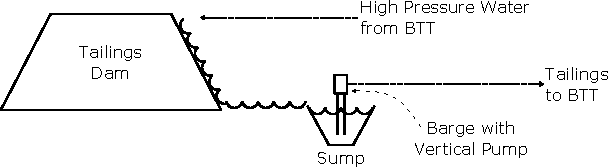
\includegraphics[width=4.3in]{TailingsDam.pdf}
	\caption{Flowsheet of the Tailings Dam operations.}
	\label{fig:TailingsDam}
\end{figure*}

An overview of the BTT plant's flowsheet is presented in Fig. \ref{fig:BTTFlowSheet}. It uses a large vibrating screen to remove plant debris that unavoidably make its way into the tailings feed. A surge tank is then used to stabilise the tailings density, followed by a hydrocyclone and thickener for dewatering. 

\begin{figure*}[b!]
	\centering
	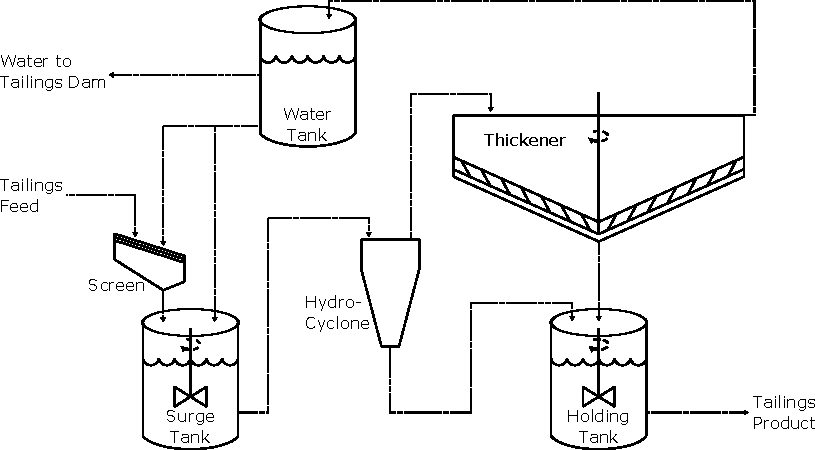
\includegraphics[width=5.2in]{BTTDetailed.pdf}
	\caption{Flowsheet of the BTT plant.}
	\label{fig:BTTFlowSheet}
\end{figure*}


%PlantDetailed.tex
The overall performance of the plant is measured on the stability of the tailings from the holding tank. Since the feed density to a hydrocyclone has by far the largest impact on the hydrocyclone efficiency \citep{Ntengwe2011}, compounding improvements in both hydrocyclone and thickener efficiencies can be expected from stabilising the surge tank density. Hence, the work presented here focuses on improving the stability of the surge tank density. 

\begin{figure}[t!]
	\centering
	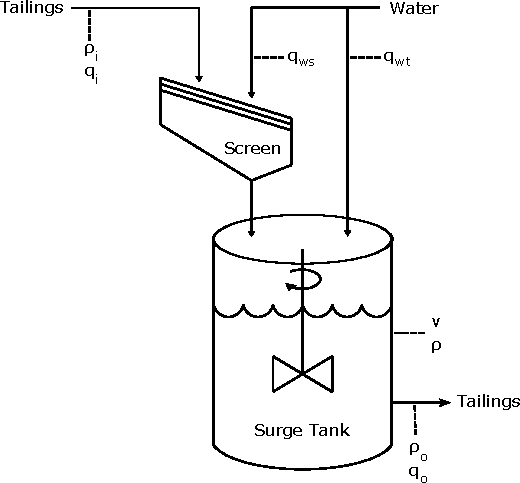
\includegraphics[width=3in]{SurgeTankDrawingNew.pdf}
	\caption{BTT surge tank.}
	\label{fig:BTTSurgeTank}
\end{figure}

\begin{table}[bp]
	\centering
	\caption{A description of the surge tank process variables.}
	\label{Table:ProcessVariables}
	\begin{tabular}{lll}
		\hline 
		Parameter 	&  Units & Description \tabularnewline
		\hline
		$q_{i}$ 	& m\textsuperscript{3}/h 	& 	Feed from tailings dam.\tabularnewline
		$q_{w}$ 	& m\textsuperscript{3}/h 	& 	Total water to surge tank.\tabularnewline
		$q_{o}$ 	& m\textsuperscript{3}/h 	& 	Tailings feed from surge tank.\tabularnewline
		$\rho_i$	& tons/m\textsuperscript{3}	&	Input density from tailings dam.\tabularnewline
		$\rho$		& tons/m\textsuperscript{3}	&	Density in surge tank.\tabularnewline
		$\rho_o$	& tons/m\textsuperscript{3}	&	Output density from surge tank.\tabularnewline
		$v$			& m\textsuperscript{3}		&	Volume in surge tank.\tabularnewline
		\hline
	\end{tabular}
\end{table}


%===============================================================================
\section{Dynamic Modelling}\label{Section:DynamicModelling}
%///////////////////////////////////////////////////////////////////////////////
\subsection{Non-Linear state space model}
A non-linear model of the surge tanks was developed to assess how effective different control strategies are at rejecting the typical input density disturbances from the tailing dam. Fig. \ref{fig:BTTSurgeTank} presents a simplified schematic diagram of the surge tank, with all relevant process variables labelled. The input flow rate, water flow rate, and output flow rate are respectively $q_i$, $q_w$, and $q_o$.The tank volume, derived from a tank level measurement, is $v$, and the input density, the density in the tank, and the output density are $\rho_i$, $\rho$, and $\rho_o$.

Assuming perfect mixing, i.e. $\rho = \rho_o$, and conservation of mass the rate of accumulation of mass in the surge tank is 
\begin{equation}
	\frac{d\rho v}{dt} = \rho_iq_i + q_w - \rho q_o .
\label{eq:MassBalance}
\end{equation}

The differential term on the left is expanded using the chain rule
\begin{equation}
v\frac{d\rho}{dt} + \rho\frac{dv}{dt}= \rho_iq_i + q_w - \rho q_o .
\label{eq:AxpandedMassBalance}
\end{equation}

%By not assuming constant volume, the model expresses the dynamics of the surge tank volume when investigating control strategies that use the tank volume to dampen input density disturbances.

Assuming no volume change during mixing, which is a reasonable assumption when modeling slurry dynamics \citep{Dontsov2014}, the volume in the surge tank will be conserved, and the rate of change of volume in the surge tank can be expressed as
\begin{equation}
\frac{dv}{dt} = q_i + q_w - q_o.
\label{eq:VolumeDynamics}
\end{equation}

Substituting (\ref{eq:VolumeDynamics}) into (\ref{eq:AxpandedMassBalance}) gives the rate of accumulation of density independent of the rate of change in volume 
\begin{equation}
\frac{d\rho}{dt} = \frac{q_i\rho_i - \rho(q_i + q_w) + q_w}{v}.				 
\label{eq:NonLinearDensityDynamics}
\end{equation}

The non-linear model of the surge tank follows from (\ref{eq:VolumeDynamics}) and (\ref{eq:NonLinearDensityDynamics})

\begin{gather}
	\begin{bmatrix} \dot{v}\\ \dot{\rho} \end{bmatrix}
	=
	\begin{bmatrix} q_i + q_w - q_o \\ \frac{1}{v}(q_i\rho_i - \rho(q_i + q_w) + q_w) \end{bmatrix},
\label{eq:NonLinearStateSpace}
\end{gather}
which is of the form:
\begin{equation}
\boldsymbol{\dot{x}} = \boldsymbol{f}(\boldsymbol{x}, \boldsymbol{u}, \boldsymbol{d}).				 
\label{eq:NonLinearStateSpaceForm}
\end{equation}
For this problem, the elements of the state vector $\boldsymbol{x}$ is $v$ and $\rho$, the elements of the input vector  $\boldsymbol{u}$ are $q_i$ and $q_w$, and the elements of the disturbance vector $\boldsymbol{d}$ are $\rho_i$ and $q_o$.

%///////////////////////////////////////////////////////////////////////////////
\subsection{Model Validation}\label{sec:ModelValidation}
The model is validated using a 10 hour long dataset collected from the plant while it was under normal operation, i.e. while the plant was not under start-up or shut-down. Figure \ref{fig:DataSet} provides an overview of this dataset.
\begin{figure}[t!]
	\centering
	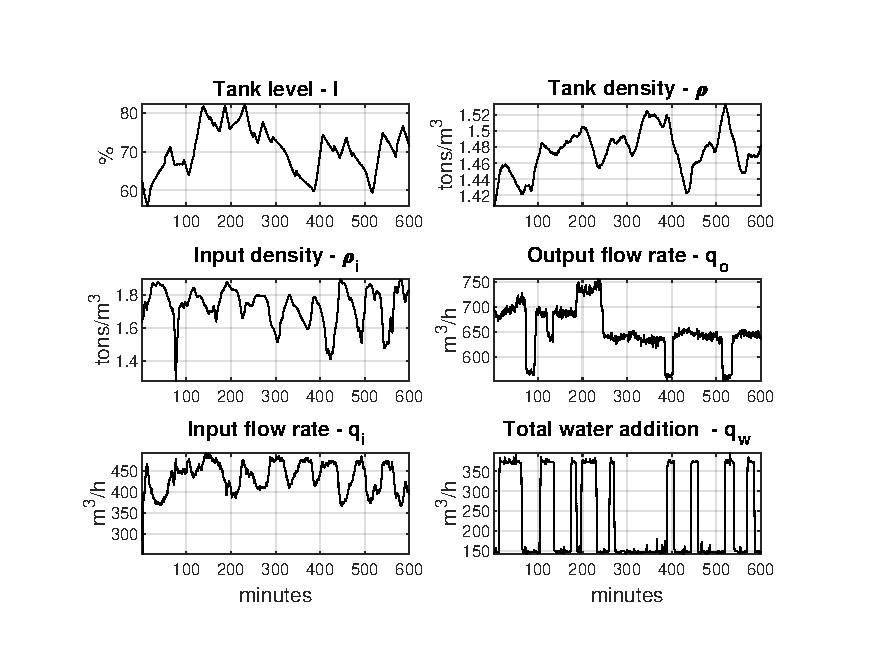
\includegraphics[trim={0.8cm, 0.8cm, 0.8cm, 0.8cm}, clip, width=\textwidth]{data_inspection.pdf}
	\caption{Data from time period when plant during normal operation.}
	\label{fig:DataSet}
\end{figure}

The non-linear model, presented in (\ref{eq:NonLinearStateSpace}), was used to generate a simulated response to the inputs and disturbances from this dataset. This simulated response is presented in Figure \ref{fig:ModelValidationNL}.
\begin{figure}[t!]
	\centering
	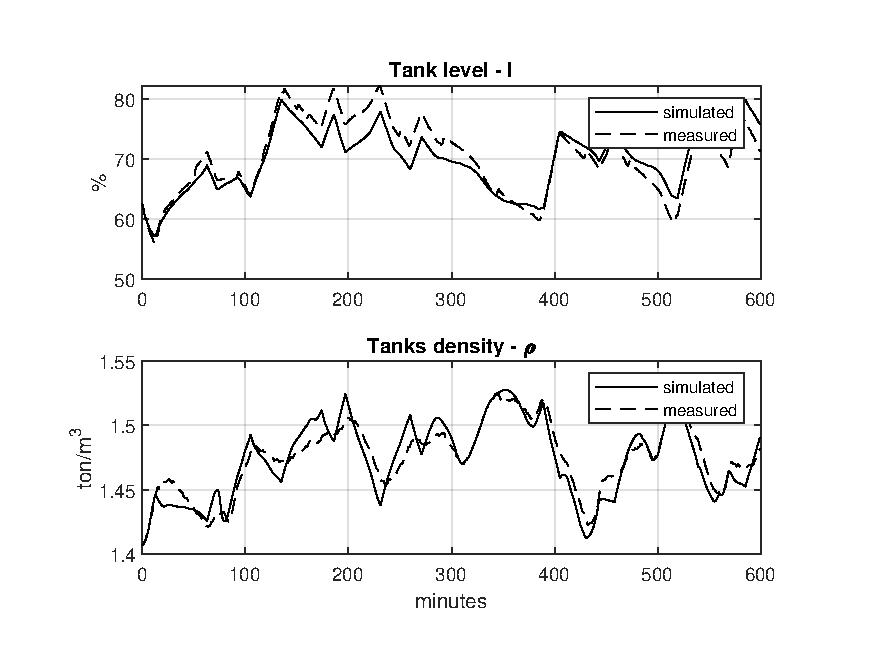
\includegraphics[trim={0.8cm, 0.8cm, 0.8cm, 0.8cm}, clip, width=\textwidth]{model_validation_nl.pdf}
	\caption{Validation of the non-linear model.}
	\label{fig:ModelValidationNL}
\end{figure}

%///////////////////////////////////////////////////////////////////////////////
%\subsection{Linear approximation}
%A linear approximation of a system is generally useful in that it allows for applying the well developed theory on linear systems \citep{Skogestad2005} to gain insights into the system's dynamic behaviour. An in-depth exploration of the surge tank's dynamics is not presented here, however, the interested reader is referred to (XXXLuke's PaperXXX) wherein is included a input/output controllability analysis for this system. The linear approximation for the surge tank's dynamics is described here and used in the section that follows to motivate for the use of a non-linear model predictive control solution. 
%
%In general, a linear approximation for a non-linear system can be obtained by a Taylor series expansion of functions \citep{Seborg2011}. Consider the function $f(x)$ of a single variable $x$. The Taylor series expansion of $f(x)$ about the point $x = \bar{x}$ is 
%\begin{align}
%\begin{split}
%f(x) &= f(\bar{x}) + \left.\frac{\partial f}{\partial x}\right\rvert_{\bar{x}} \delta x + \frac{1}{2}\left.\frac{\partial^2 f}{\partial x^2}\right\rvert_{\bar{x}} \delta x^2 + 
%\frac{1}{6}\left.\frac{\partial^3 f}{\partial x^3}\right\rvert_{\bar{x}} \delta x^3 +  ... \\
%&= \sum_{n=0}^{\infty}\frac{1}{n!} \left.\frac{\partial^n f}{\partial x^n}\right\rvert_{\bar{x}}\delta x^n ,
%\end{split}
%\label{eq:Taylor}
%\end{align}
%with $\delta x = x - \bar{x}$. For $x$ close to $\bar{x}$ the higher order terms in (\ref{eq:Taylor}) will be approximately zero. Hence, a linear approximation of $f(x)$ is obtained by discarding the higher order terms
%\begin{equation}
%f(x) \cong f(\bar{x}) + \left.\frac{\partial f}{\partial x}\right\rvert_{\bar{x}} \delta x . 
%\label{eq:LinearTaylor}
%\end{equation}
%
%The expression for the accumulation of volume in (\ref{eq:VolumeDynamics}) is already linear, therefore, a linear approximation of the surge tank requires only a Taylor series expansion of (\ref{eq:NonLinearDensityDynamics}). Taking the functional form
%\begin{gather}
%	\frac{d\rho}{dt} = f_{\rho}(q_i, q_w, q_o, \rho_i, \rho, v),
%\end{gather}
%and applying a multivariate extension of (\ref{eq:LinearTaylor}) about the nominal steady-state operating point $\bar{x} = (\bar{q}_i, \bar{q}_w, \bar{\rho}_i, \bar{\rho}, \bar{v})$ gives:
%\begin{align}
%	\begin{split}
%	&f_{\rho}(q_i, q_w, q_o, \rho_i, \rho, v) \cong \left. f_{\rho}(\bar{x}) + \frac{\partial f_{\rho}}{\partial q_i}\right\rvert_{\bar{x}}\delta q_i + \left.\frac{\partial f_{\rho}}{\partial q_w}\right\rvert_{\bar{x}}\delta q_w + \left.\frac{\partial f_{\rho}}{\partial q_o}\right\rvert_{\bar{x}}\delta q_o + \\
%	&\phantom{f(q_i, q_w, q_o, \rho_i, \rho, v) \cong}\left.\frac{\partial f_{\rho}}{\partial \rho_i}\right\rvert_{\bar{x}}\delta \rho_i + \left.\frac{\partial f_{\rho}}{\partial \rho}\right\rvert_{\bar{x}}\delta \rho + \left.\frac{\partial f_{\rho}}{\partial v}\right\rvert_{\bar{x}}\delta v\\ 
%	\\
%	&\phantom{f_{\rho}(q_i, q_w, q_o, \rho_i, \rho, v)} \cong f_{\rho}(\bar{x}) + \frac{\bar{\rho}_i - \bar{\rho}}{\bar{v}}\delta q_i + \frac{1 - \bar{\rho}}{\bar{v}}\delta q_w + \frac{\bar{q}_i}{\bar{v}}\delta \rho_i \\
%	&\phantom{f_{\rho}(q_i, q_w, q_o, \rho_i, \rho, v) \cong } - \frac{\bar{q}_i + \bar{q}_w}{\bar{v}}\delta \rho -  \frac{\bar{q}_i\bar{\rho}_i + \bar{q}_w - (\bar{q}_i + \bar{q}_w)\bar{\rho}}{\bar{v}^2} \delta v .
%	\end{split}
%	\label{eq:DensityLinear}
%\end{align}
%
%By definition, at steady state
%\begin{align}
%\begin{split}
%	\bar{q}_i + \bar{q}_w - \bar{q}_o = 0 \\
%	\text{and} \\
%	\bar{q}_i\bar{\rho}_i + \bar{q}_w - \bar{q}_o\bar{\rho} = 0,
%\end{split}
%\end{align}
%and (\ref{eq:DensityLinear}) reduces to: 
%\begin{equation}
%	f_{\rho}(q_i, q_w, q_o, \rho_i, \rho, v) \cong f_{\rho}(\bar{x}) +\frac{\bar{\rho}_i - \bar{\rho}}{\bar{v}}\delta q_i + \frac{1 - \bar{\rho}}{\bar{v}}\delta q_w + \frac{\bar{q}_i}{\bar{v}}\delta \rho_i - \frac{\bar{q}_o }{\bar{v}}\delta \rho .
%	\label{eq:DensityLinearSimple}	
%\end{equation}
%
%A linear approximation of the surge tank model follows from (\ref{eq:VolumeDynamics}) and (\ref{eq:DensityLinearSimple}), presented here in state space form:
%\begin{align}
%	\begin{split}
%	\boldsymbol{\dot{x}} = \boldsymbol{A}\boldsymbol{x} + \boldsymbol{B}\boldsymbol{u} \\
%	\boldsymbol{y} = \boldsymbol{C}\boldsymbol{x}\\
%	\text{with} \\
%	\boldsymbol{\dot{x}} = \begin{bmatrix} \frac{dv}{dt} \\ \frac{d\rho}{dt} \end{bmatrix}, \boldsymbol{x} = \begin{bmatrix} v \\ \rho \end{bmatrix}, \boldsymbol{u} = \begin{bmatrix} q_i \\ q_w \\ q_o \\ \rho_i \end{bmatrix}, \\ 
%	\boldsymbol{A} = \begin{bmatrix} 0 & 0 \\ 0 & -\frac{\bar{q}_o}{\bar{v}}  \end{bmatrix}, 
%	\boldsymbol{B} = \begin{bmatrix} 1 & 1 & -1 & 0 \\ \frac{\bar{\rho}_i - \bar{\rho}}{\bar{v}} & \frac{1 - \bar{\rho}}{\bar{v}} & 0 & \frac{\bar{q}_o}{\bar{v}} \end{bmatrix}, and \hspace{2mm}
%	\boldsymbol{C} = \begin{bmatrix} 1 & 0 \\ 0 & 1  \end{bmatrix}. \\
%	\end{split}
%	\label{eq:LinearModel}
%\end{align}

%///////////////////////////////////////////////////////////////////////////////
\subsection{Model Predictive Control}\label{sec:MPC}
The MPC controller can be described as:
\begin{equation}\label{eq:mpc_obj}
\begin{array}{l}
\underset{u_{k|k},...,u_{k|k+N_c}}{\min} J\left(u,x_{k|k}\right)\\
\mathrm{s.t.}\\
\begin{array}{l}
x\in \mathcal{X} \triangleq \left\lbrace \left.x\in\mathbb{R}^{N_x\times N_p}\right|x_l\leq x\leq x_h \right\rbrace\\
u\in \mathcal{U} \triangleq \left\lbrace \left.u\in\mathbb{R}^{N_u\times N_c}\right|u_l\leq u\leq u_h \right\rbrace\\
y\in \mathcal{Y} \triangleq \left\lbrace \left.y\in\mathbb{R}^{N_y\times N_p}\right|y_l\leq y\leq y_h \right\rbrace\\

x(k|k) \triangleq \mathrm{Initial~state}
\end{array}\\
\left.
\begin{array}{ll}
x_{k+i+1|k} &= f\left(x_{k+i|k},u_{k+i|k}\right) \\
y_{k+i|k} &= h\left(x_{k+i|k},u_{k+i|k}\right)\\
\end{array}\right\rbrace \forall i=1,2,...,N_c\\
\left.
\begin{array}{ll}
x_{k+i+1|k} &= f\left(x_{k+i|k},u_{k+N_c|k}\right) \\
y_{k+i|k} &= h\left(x_{k+i|k},u_{k+N_c|k}\right)\\
\end{array}\right\rbrace \forall i=N_c+1,N_c+2,...,N_p\\
\end{array}
\end{equation}
where $N_p$ is the prediction horizon, $N_c$ is the control horizon. The cost function is defined as:
\begin{equation}
J(\cdot) = \displaystyle\sum_{i=1}^{N_p} \left\Vert y_{sp}-y_{k+i|k} \right\Vert _Q^2  + \displaystyle\sum_{i=1}^{N_c} \left\Vert\Delta u_{k+i|k} \right\Vert_R^2
\end{equation}
where $y_{sp}$ is the controlled variable set-points, and $Q$ and $R$ are the controlled and manipulated variable weighting matrices respectively. 

%///////////////////////////////////////////////////////////////////////////////
%\subsection{Linear vs non-linear}\label{sec:ModelValidation}
%Recall that the linear model in (\ref{eq:LinearModel}) was derived on the assumption that higher order, non-linear, terms in (\ref{eq:Taylor}) can be disregarded since, close to the nominal operating point $\bar{x}$, higher order terms will be approximately zero. Processes, of course, continuously deviate from their nominal operating point, and inaccuracies arising from linear model approximations can not be avoided. These inaccuracies between the true system dynamics and those predicted by the model is generally revered to as model mismatch.
%
%Considering that the vast majority of industrial model predictive control solutions rely on linear models to control non-linear processes \citep{QinAndBadgwell2003}, there seem to exist a general disregard for model mismatch. This can be explained by noting that it is comparatively cheap to develop linear models, typically by assuming that the linear dynamic responses of the system follows first order with time delay (FOPDT) transients, and by fitting FOPDT models to data obtained from step testing. Compared to a first principles approach to obtain a non-linear model a linear model obtained from step tests are markedly less complicated and time consuming. Generally, linear approximations are at least accurate to the direction of relationships between model inputs and outputs. This is considered "good enough" for control since the system can be driven towards a desired operating point. Moreover, the negative effects of some model mismatch is likely never considered when a linear MPC achieves noteworthy improvements compared to the legacy control system. 
%
%A linear approximation for this surge tank model would not be sufficient, however, since the expected deviation of input density from the tailings dam would cause inversion of the direction of the relationship between input flow $q_i$ and tank density $\rho$. Consider that for the linear approximation of the surge tank model, the term in the input matrix $\boldsymbol{B}$ in (\ref{eq:LinearModel}) associated with the input flow $q_i$ will always be positive, since a constant flow of input water $q_w$ is needed to maintain the screen, which would dilute the incoming tailings and guarantee that 
%\begin{equation}
%	\frac{\bar{\rho_i} - \bar{\rho}}{\bar{v}} > 0 .
%\end{equation}
%A linear MPC relying on the model in (\ref{eq:LinearModel}) would therefore always use $q_i$ to increase $\rho$. However, the re-mining process followed at the tailings dam, described in Section \ref{sec:CircuitAnalysis}, is very unstable and results in an instantaneous input density $\rho_i$ that varies over a large range, often resulting in a scenario where $\rho_i - \rho < 0$. 
%
%This means that in the particular scenario where
%\begin{equation}
%\rho_i - \rho < 0 \text{ and } \rho < \rho_{target}, 
%\end{equation}
%the linear MPC would increase $q_i$ further driving $\rho$ away from $\rho_{target}$. Under this scenario, $\rho$ can be maintained closer to $\rho_{target}$, by decreasing the input allowing the tank level $l$ to 
%
%



%===============================================================================
%///////////////////////////////////////////////////////////////////////////////
\section{Controller Design and Simulation}\label{sec:ControllerDesignAndSimulation}



%===============================================================================
%///////////////////////////////////////////////////////////////////////////////
\section{Controller Implementation and Evaluation}\label{sec:ControllerImplementationAndEvaluation}



%===============================================================================
%///////////////////////////////////////////////////////////////////////////////



\bibliographystyle{model2-names}
\bibliography{references}

\end{document}

%%
%% End of file `elsarticle-template-2-harv.tex'.
